\documentclass{exam}
\usepackage[exos]{main}

\title{Exercices : Probabilités}
\date{3 Mai 2024}
\author{Seconde 9}

\begin{document}
\maketitle
\begin{tcolorbox}
Faire les exercices de la colonne de droite. En cas de difficulté, faire l'exercice correpondant dans la colonne de gauche.
\end{tcolorbox}
\begin{minipage}{0.45\textwidth}
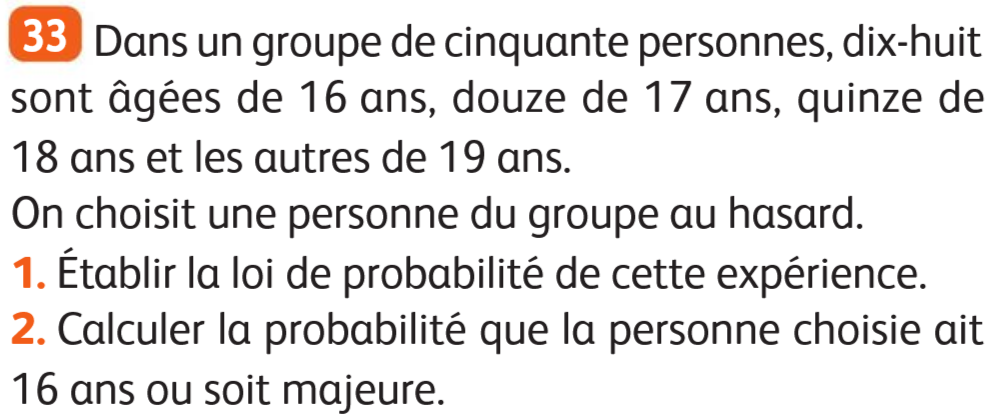
\includegraphics[width=\textwidth]{Exo33.png}
\vspace*{0.25cm}

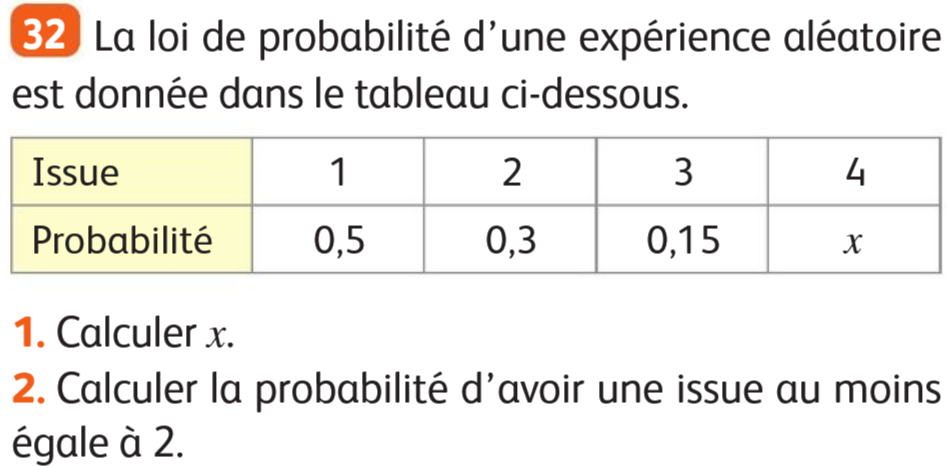
\includegraphics[width=\textwidth]{Exo32.png}
\vspace*{1.7cm}

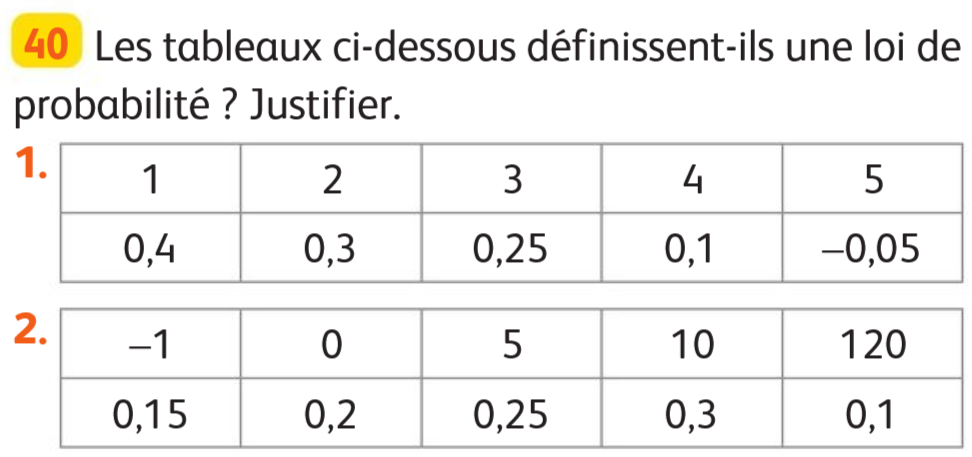
\includegraphics[width=\textwidth]{Exo40}
\end{minipage}
\hfill\vline\hfill
\begin{minipage}{0.45\textwidth}
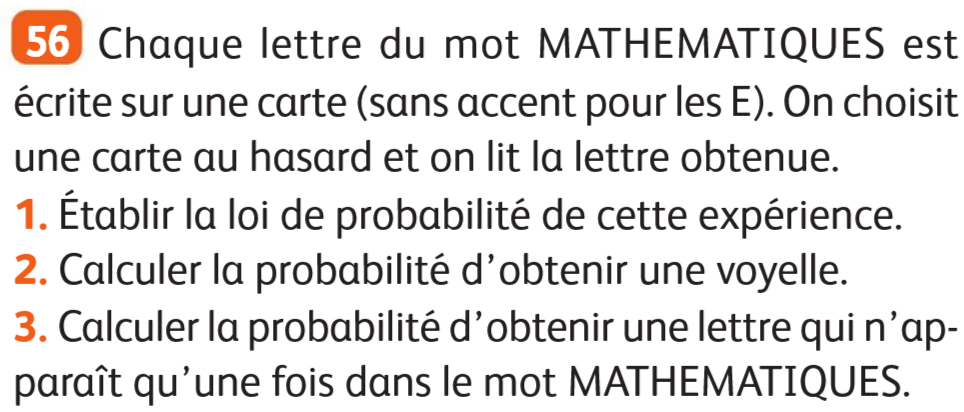
\includegraphics[width=\textwidth]{Exo56.png}
\vspace*{0.25cm}

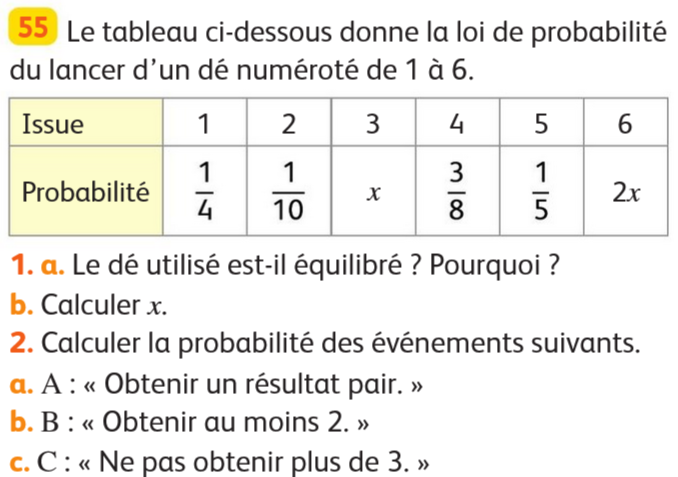
\includegraphics[width=\textwidth]{Exo55.png}
\vspace*{0.25cm}

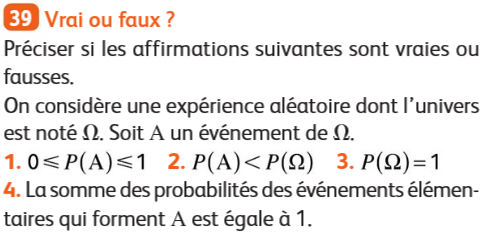
\includegraphics[width=\textwidth]{Exo39.png}
\end{minipage}
\end{document}